% !TeX program = lualatex
\documentclass[12pt]{IEEEtran}
\IEEEoverridecommandlockouts
\usepackage{fancyhdr}
\usepackage{graphicx}
\usepackage[spanish, es-tabla, es-nodecimaldot]{babel}
% \usepackage[utf8]{inputenc}
\usepackage{csquotes}
\usepackage{wrapfig}
\usepackage[l3]{csvsimple}
\usepackage{array}
\usepackage[calc, spanish]{datetime2}
\usepackage{enumitem}
% \usepackage{multicol}
\usepackage{chemformula}
\usepackage{multirow}
\usepackage{mismath}
\usepackage[export]{adjustbox}
\usepackage{nccmath}
\usepackage{amsmath}
\usepackage{amssymb}
\usepackage{mathtools}
\usepackage{amsfonts,latexsym} % para tener disponibilidad de diversos simbolos
\usepackage{enumerate}
\usepackage{empheq}
\usepackage{derivative}
\usepackage{float}
\usepackage{threeparttable}
\usepackage{ifpdf}
\usepackage{rotating}
\usepackage{stfloats}
\usepackage{tabularray}
\usepackage{url}
% \usepackage[inline]{showlabels}
\usepackage{kantlipsum}
\usepackage{siunitx}
\usepackage{makecell}%To keep spacing of text in tables
\setcellgapes{2pt}%parameter for the spacing in tables
\usepackage{afterpage}
\usepackage[
  sorting=none,
  backend=biber,
  style=ieee,
  % bibstyle = authoryear,
  citestyle=numeric-comp,
]{biblatex}
\usepackage{hyperref}
\usepackage{cleveref}
\crefname{table}{tabla}{tablas} % Table's cross-reference name
\crefname{equation}{ec.}{ecs.} %
\newcommand\crefrangeconjunction{--}
\newcommand\crefpairconjunction{~y~}
\providecommand{\abs}[1]{\lvert#1\rvert}
%%%%%%%%%%%%%%%%%%%%%%%%%%%%%%%%%%%%%%%%%%%
%%% CREAR Y REESCRIBIR ALGUNOS COMANDOS %%%
%%%%%%%%%%%%%%%%%%%%%%%%%%%%%%%%%%%%%%%%%%%
\newcolumntype{P}[1]{>{\centering\arraybackslash}p{#1}}  %% Se crea un nuevo tipo de columna llamada P.
\newcommand{\tabitem}{~~\llap{\textbullet}~~}
\newcommand{\ctt}{\centering\scriptsize\textbf} %%\ctt abrevia el comando \centering\scriptsize\textbf
\newcommand{\dtt}{\scriptsize\textbf} %%\dtt abrevia el comando \scriptsize\textbf
\renewcommand\IEEEkeywordsname{Palabras clave}

%%%%%%%%%%%%%%%%%%%%%%%%%%%%%%%%%%%%%%%%%%%
\graphicspath{ {figs/} {logos/}}  %%Ruta donde se encuentran las imágenes, que esté vacio indica que las imagenes están dentro de la misma carpeta que contiene el archivo .tex

\sisetup{
  output-decimal-marker = {.},
  uncertainty-mode = separate,
}
% adjust as needed
\addtolength{\footskip}{0\baselineskip}
\addtolength{\textheight}{-1\baselineskip}

%%%%%%%%%%%%%%%%%%%%%%%%%%%%%%%%
%%%%% INICIO DEL DOCUMENTO %%%%%
%%%%%%%%%%%%%%%%%%%%%%%%%%%%%%%%

\addbibresource{AnalisisDePlasmaBNDepositadoPorRF.bib}

\DTMsavedate{duedate}{2024-03-25}% Año-Mes-Día -> Fecha de entrega
\DTMnewdatestyle{usvardate}{%
  \renewcommand{\DTMdisplaydate}[4]{%
    \DTMMonthname{##2}\nobreakspace% Mes
    \number##1% Año
  }%
  \renewcommand{\DTMDisplaydate}{\DTMdisplaydate}%
}

\DeclareSIUnit{\min}{min}
\DeclareSIUnit{\Torr}{Torr}
\DeclareSIUnit{\mTorr}{mTorr}

\begin{document}
%%%%%%%%%%%%%%%%%%%%%%%%%%%%
%%% TÍTULO DEL DOCUMENTO %%%
%%%%%%%%%%%%%%%%%%%%%%%%%%%%

\title{Análisis de plasma de nitruro de boro \ch{BN} por espectrometría de emisión óptica obtenido por rf Magnetron Sputtering}

%%%%%%%%%%%%%%%%%%%%%%%%%%%
%%%%%%%%% AUTORES %%%%%%%%%
%%%%%%%%%%%%%%%%%%%%%%%%%%%
\author{\IEEEauthorblockN{Jesús Diego Gómez Garnica, Marcos López Merino}\\
	\IEEEauthorblockA{\textbf{Profesor}: Julio César Cruz Cárdenas}\\
	\IEEEauthorblockN{\DTMusedate{duedate}}}

%%%%%%%%%%%%%%%%%%%%%%%%%%%
\twocolumn[
	\begin{@twocolumnfalse}
		\maketitle
		\begin{abstract}
			En este trabajo se utilizó la técnica de espectrometría de emisión óptica (OES) para analizar la composición del plasma generado durante el depósito de una película de nitruro de boro \ch{BN} mediante la técnica de \emph{Radio Frequency Magnetron Sputtering}. El espectro de emisión se registró a una altura de \qty{5}{\cm} sobre el blanco, en su región central, a intervalos regulares de tiempo, con el objetivo de construir una base de datos para su análisis posterior. Con base en el conocimiento previo de los elementos esperados en el plasma, las líneas de emisión observadas se compararon con la base de datos del NIST, lo que permitió identificar la presencia de nitrógeno, argón y boro durante el proceso de deposición.
		\end{abstract}

		\begin{IEEEkeywords}
			Espectometría, rf magnetron sputtering, plasma
		\end{IEEEkeywords}
	\end{@twocolumnfalse}
	\vspace{1cm}
]

%%%%%%%%%%%%%%%%%%%%%%
%\IEEEpeerreviewmaketitle
%%%%%%%%%%%%%%%%%%%%%%%%%%%%%%%%%%%%%
%%% PRIMERA SECCIÓN DEL DOCUMENTO %%%
%%%%%%%%%%%%%%%%%%%%%%%%%%%%%%%%%%%%%
\section{Introducción}

Las películas delgadas son capas de uno o más materiales con espesores que van desde unos cuantos nanómetros hasta varios micrómetros. Estas pueden encontrarse en aplicaciones tan diversas como revestimientos antirreflejantes para anteojos o componentes funcionales en chips de computadoras. Su ventaja radica en la combinación de las propiedades superficiales de la película delgada con las propiedades del material subyacente, lo que mejora las características químicas, mecánicas o eléctricas, entre otras.

Existen múltiples técnicas para la fabricación de estas películas, entre ellas la electrodeposición (\emph{electroplating}), la evaporación, la pulverización catódica (\emph{sputter deposition}), la deposición química de vapor  (CVD, por sus siglas en inglés) y combinaciones de estas. En este trabajo se emplea la pulverización catódica por radiofrecuencia (\emph{rf sputtering}), una técnica que permite la deposición de materiales dieléctricos.

La pulverización catódica por radiofrecuencia (rf) opera a frecuencias superiores a \qty{50}{\kHz}. En este régimen, los iones no poseen la movilidad suficiente para establecer una descarga continua, como ocurre en en el \emph{sputtering DC}. Sin embargo, los electrones sí adquieren la energía necesaria para provocar colisiones ionizantes en el gas entre los electrodos, lo que da lugar a la formación de un plasma.
Una de las principales ventajas del \emph{sputtering rf} es la posibilidad de utilizar blancos no conductores. Esto se debe a que el potencial aplicado oscila, permitiendo que, durante cada medio ciclo, los iones del plasma sean acelerados hacia la superficie del blanco con la energía suficiente para provocar la pulverización. En el medio ciclo opuesto, los electrones del plasma alcanzan la superficie, neutralizando la carga acumulada e impidiendo la formación de un potencial estático.
Las frecuencias típicas utilizadas en rf se encuentran en el rango de \qtyrange[range-units=single]{0.5}{30}{\MHz}, siendo \qty{13.56}{\MHz} la más empleada comercialmente.\cite{antaritagutierrezSintesisPeliculasDelgadas2017,mattoxChapter7Physical2010}
No obstante, una desventaja importante al emplear esta técnica con materiales semiconductores o dieléctricos es que estos suelen tener baja conductividad térmica, altos coeficientes de expansión térmica y una naturaleza frágil. Estas propiedades resultan problemáticas durante el proceso de rf, ya que el bombardeo iónico genera una cantidad significativa de calor y grandes gradientes térmicos, lo cual puede inducir tensiones internas en el blanco e incluso provocar su fractura.

En este sentido, al ser el nitruro de boro un material dieléctrico, se buscó esta alternativa de rf para la fabricación de la película delgada; no obstante, el enfoque de este escrito no es acerca del producto de este método, sino del plasma generado por él mismo.

Los plasmas se generan suministrando energía a un gas neutro, lo que provoca la formación de portadores de carga. Los electrones e iones se producen en fase gaseosa cuando electrones o fotones con suficiente energía colisionan con los átomos y moléculas neutros del gas de alimentación (ionización por impacto electrónico o fotoionización). Existen diversas maneras de suministrar la energía necesaria para la generación de plasma a un gas neutro, en este caso a través de rf.\cite{mattoxChapter7Physical2010}

Para estudiar la composición del plasma es necesario hacerlo a través de la espectrometría de emisión óptica o \emph{Optical Emission Spectrometry} (OES), una técnica espectroscópica que analiza las longitudes de ondas de los fotones emitidos por los átomos o moléculas durante su transición desde un estado de inferior energía. Este espectro permite identificar y cuantificar los elementos e la muestra, siendo de gran utilidad en industrias como la metalurgia y la petroquímica.\cite{QueEsAnalisis,AnalisisPorEmision2025}

\section{Procedimiento experimental}

Mediante la técnica de \emph{OES} se estudió la composición del plasma
generado durante el depósito por rf de una película delgada de \ch{BN}
en sustratos de \ch{Si} y un portaobjetos de vidrio.

Los sustratos de \ch{Si} utilizados fueron de aproximadamente \qty{1}{\cm\squared}
obtenidos de una oblea (\emph{wafer}) de 2'' de este material de la marca \emph{TED PELLA}
a los que se les realizó una limpieza con etanol
para eliminar cualquier residuo y contaminación adquiridos durante su manipulación.
Posteriormente, en una solución de jabón industrial y agua,
se sometieron a un baño ultrasónico durante \qty{15}{\min} para una limpieza profunda.

Posteriormente, se colocó cada uno de los sustratos en el portasustratos
como se muestra en la \cref{fig:portasustratos-setup}.

\begin{figure}[htb]
	\centering
	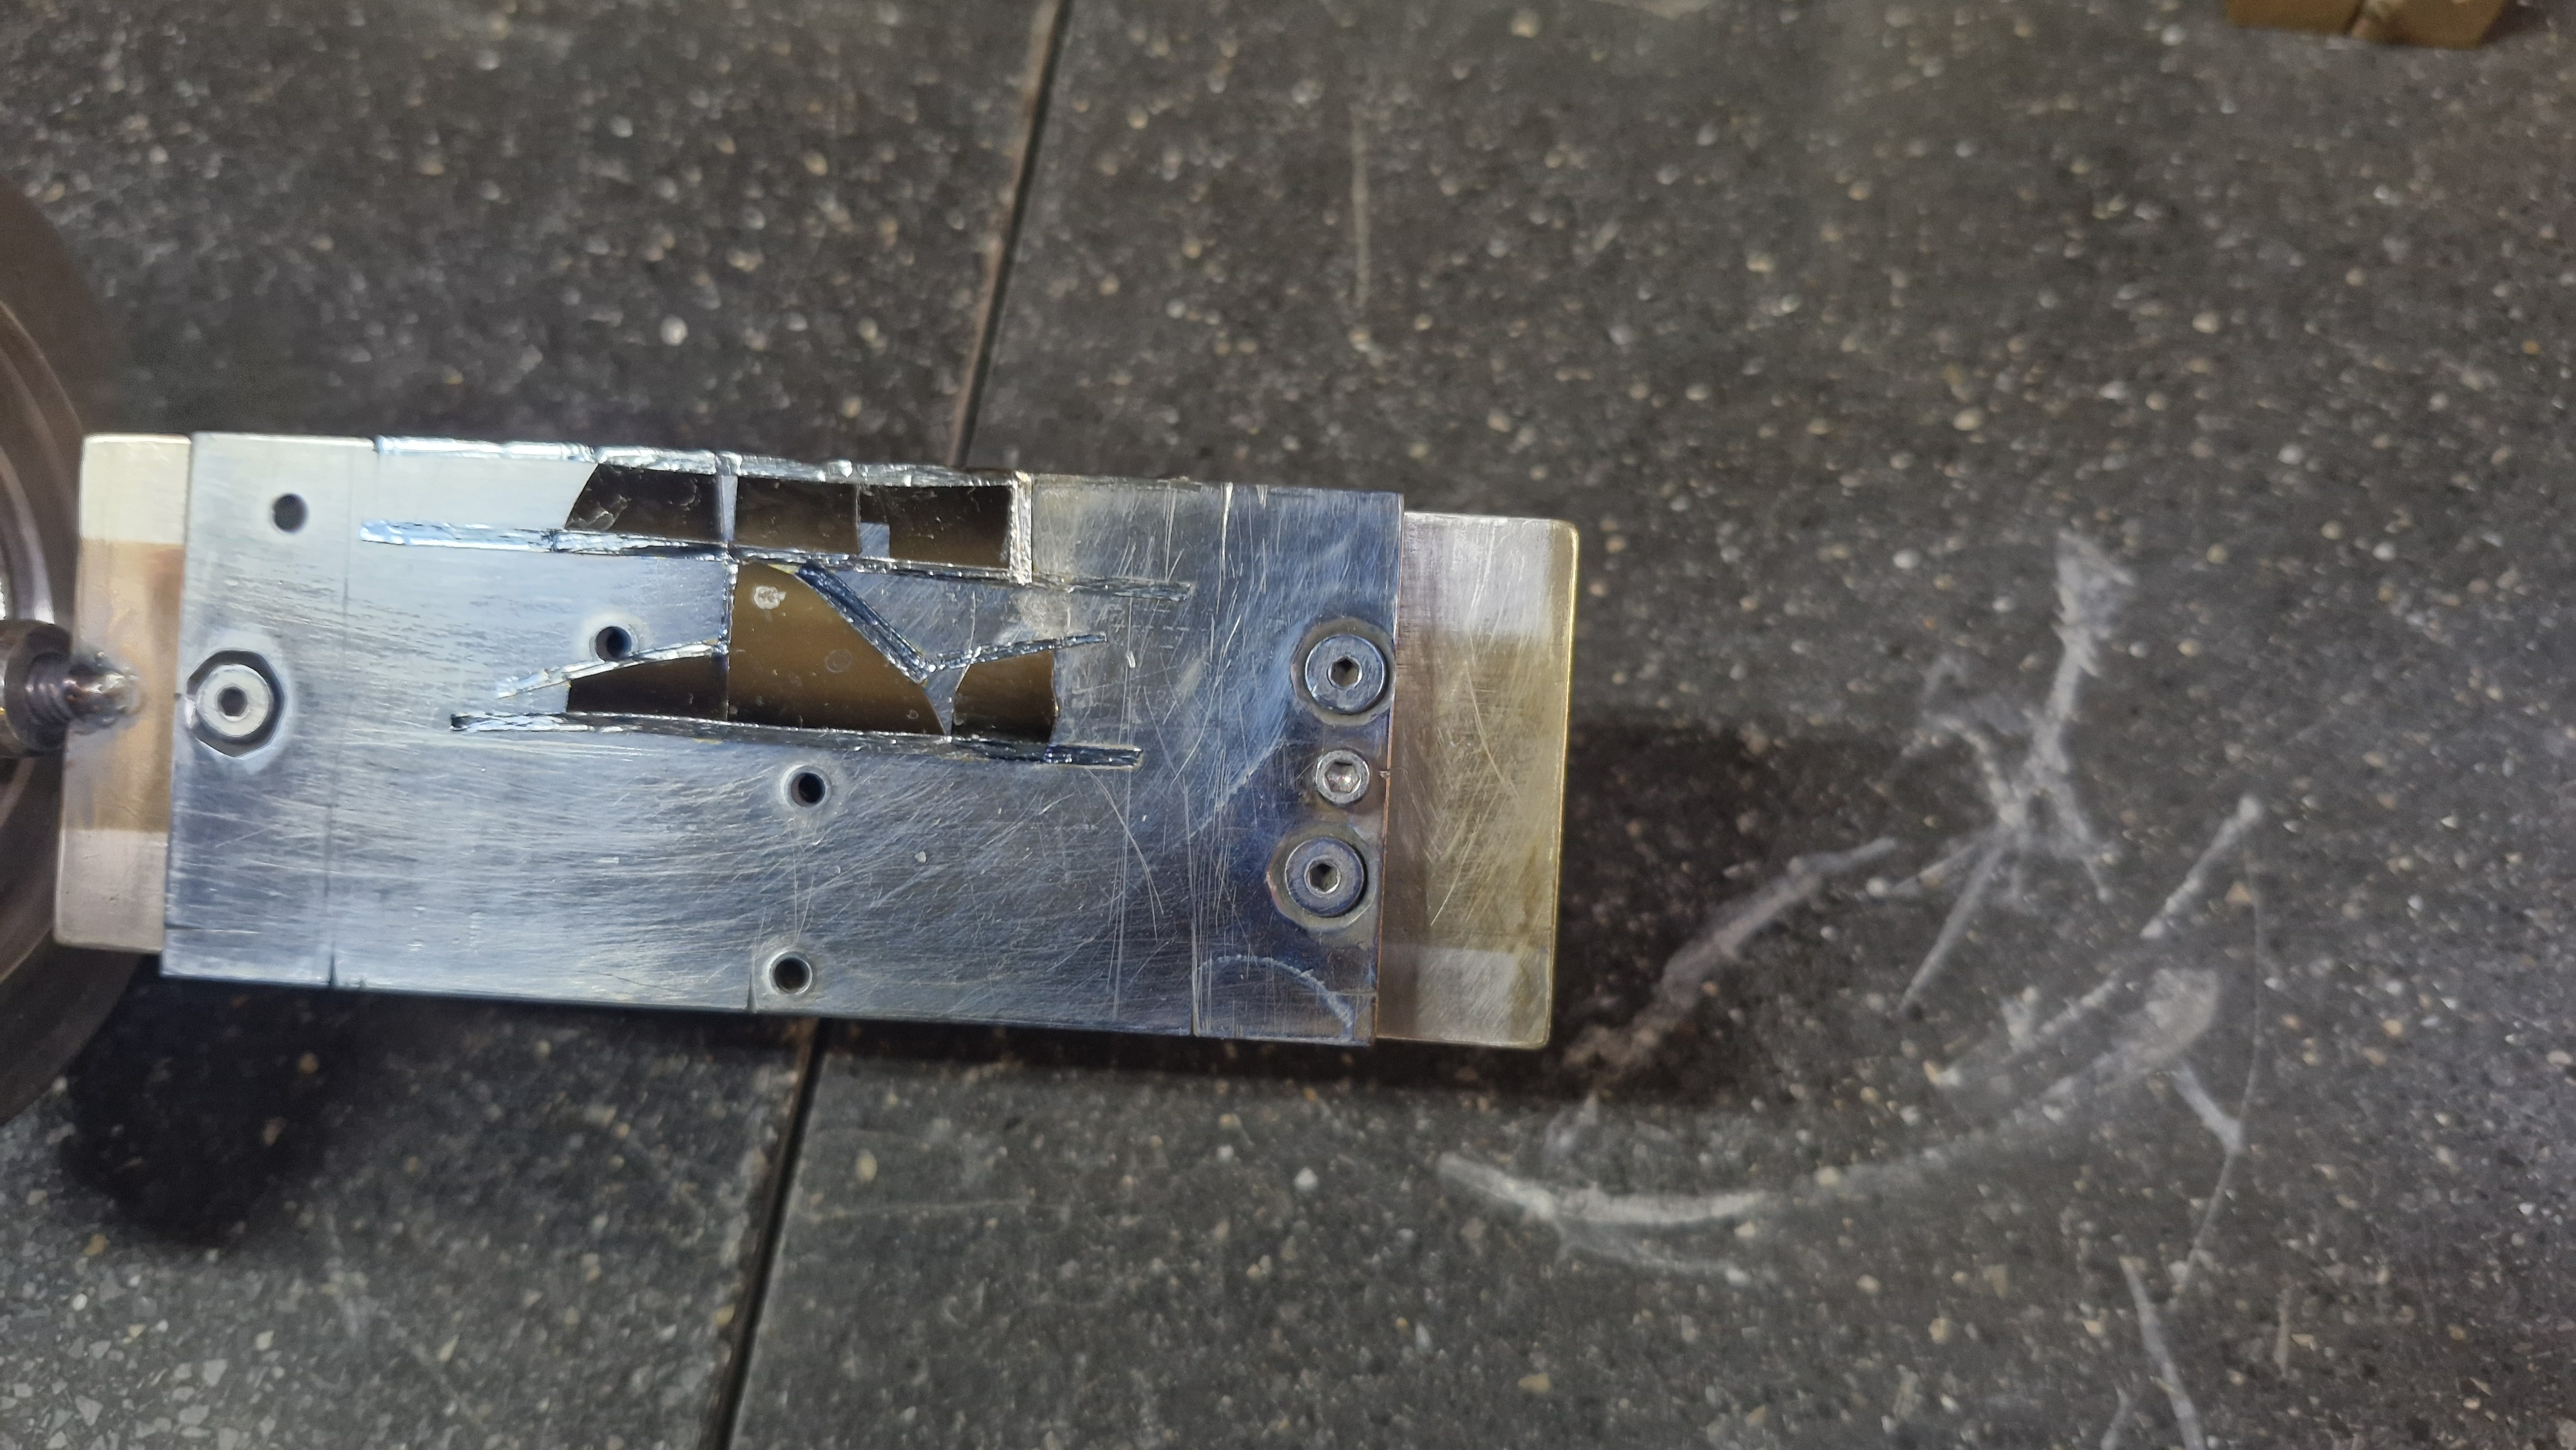
\includegraphics[width=\linewidth, trim={0 20cm 50cm 20cm},clip]{portasustratos.jpg}
	\caption{Portasustratos con sustratos de \ch{Si}.}
	\label{fig:portasustratos-setup}
\end{figure}

\subsection{Medición de Espectros}

Para la medición de los espectros de emisión se utilizó un un espectrómetro de fibra óptica
de la marca \emph{Avantes}, modelo \emph{AvaSpec-Dual} en conjunto con el software
\emph{AvaSoft-8}, el cual permite la adquisición de datos espectrales en tiempo real.
Este espectrométro cuenta con un rango de longitudes de onda de \qtyrange{200}{900}{\nm},
lo cual lo hace adecuado para la identificación de líneas de emisión
de los elementos presentes en el plasma generado durante el proceso de deposición.

\par
Primero se realizó un barrido a lo largo del \emph{racetrack}, realizando 10 mediciones
cada \qty{.2}{\cm}, para determinar la posición óptima del espectrómetro.
Esta posición se definió a través de la comparación de los espectros
obtenidos en diferentes puntos del \emph{racetrack},
donde se observó que la mayor intensidad de emisión se encontraba en el centro del blanco,
en la posición a \qty{6}{\cm} en el \emph{racetrack}, como se muestra en la \cref{fig:espectrometro}.

\begin{figure}[htb]
	\centering
	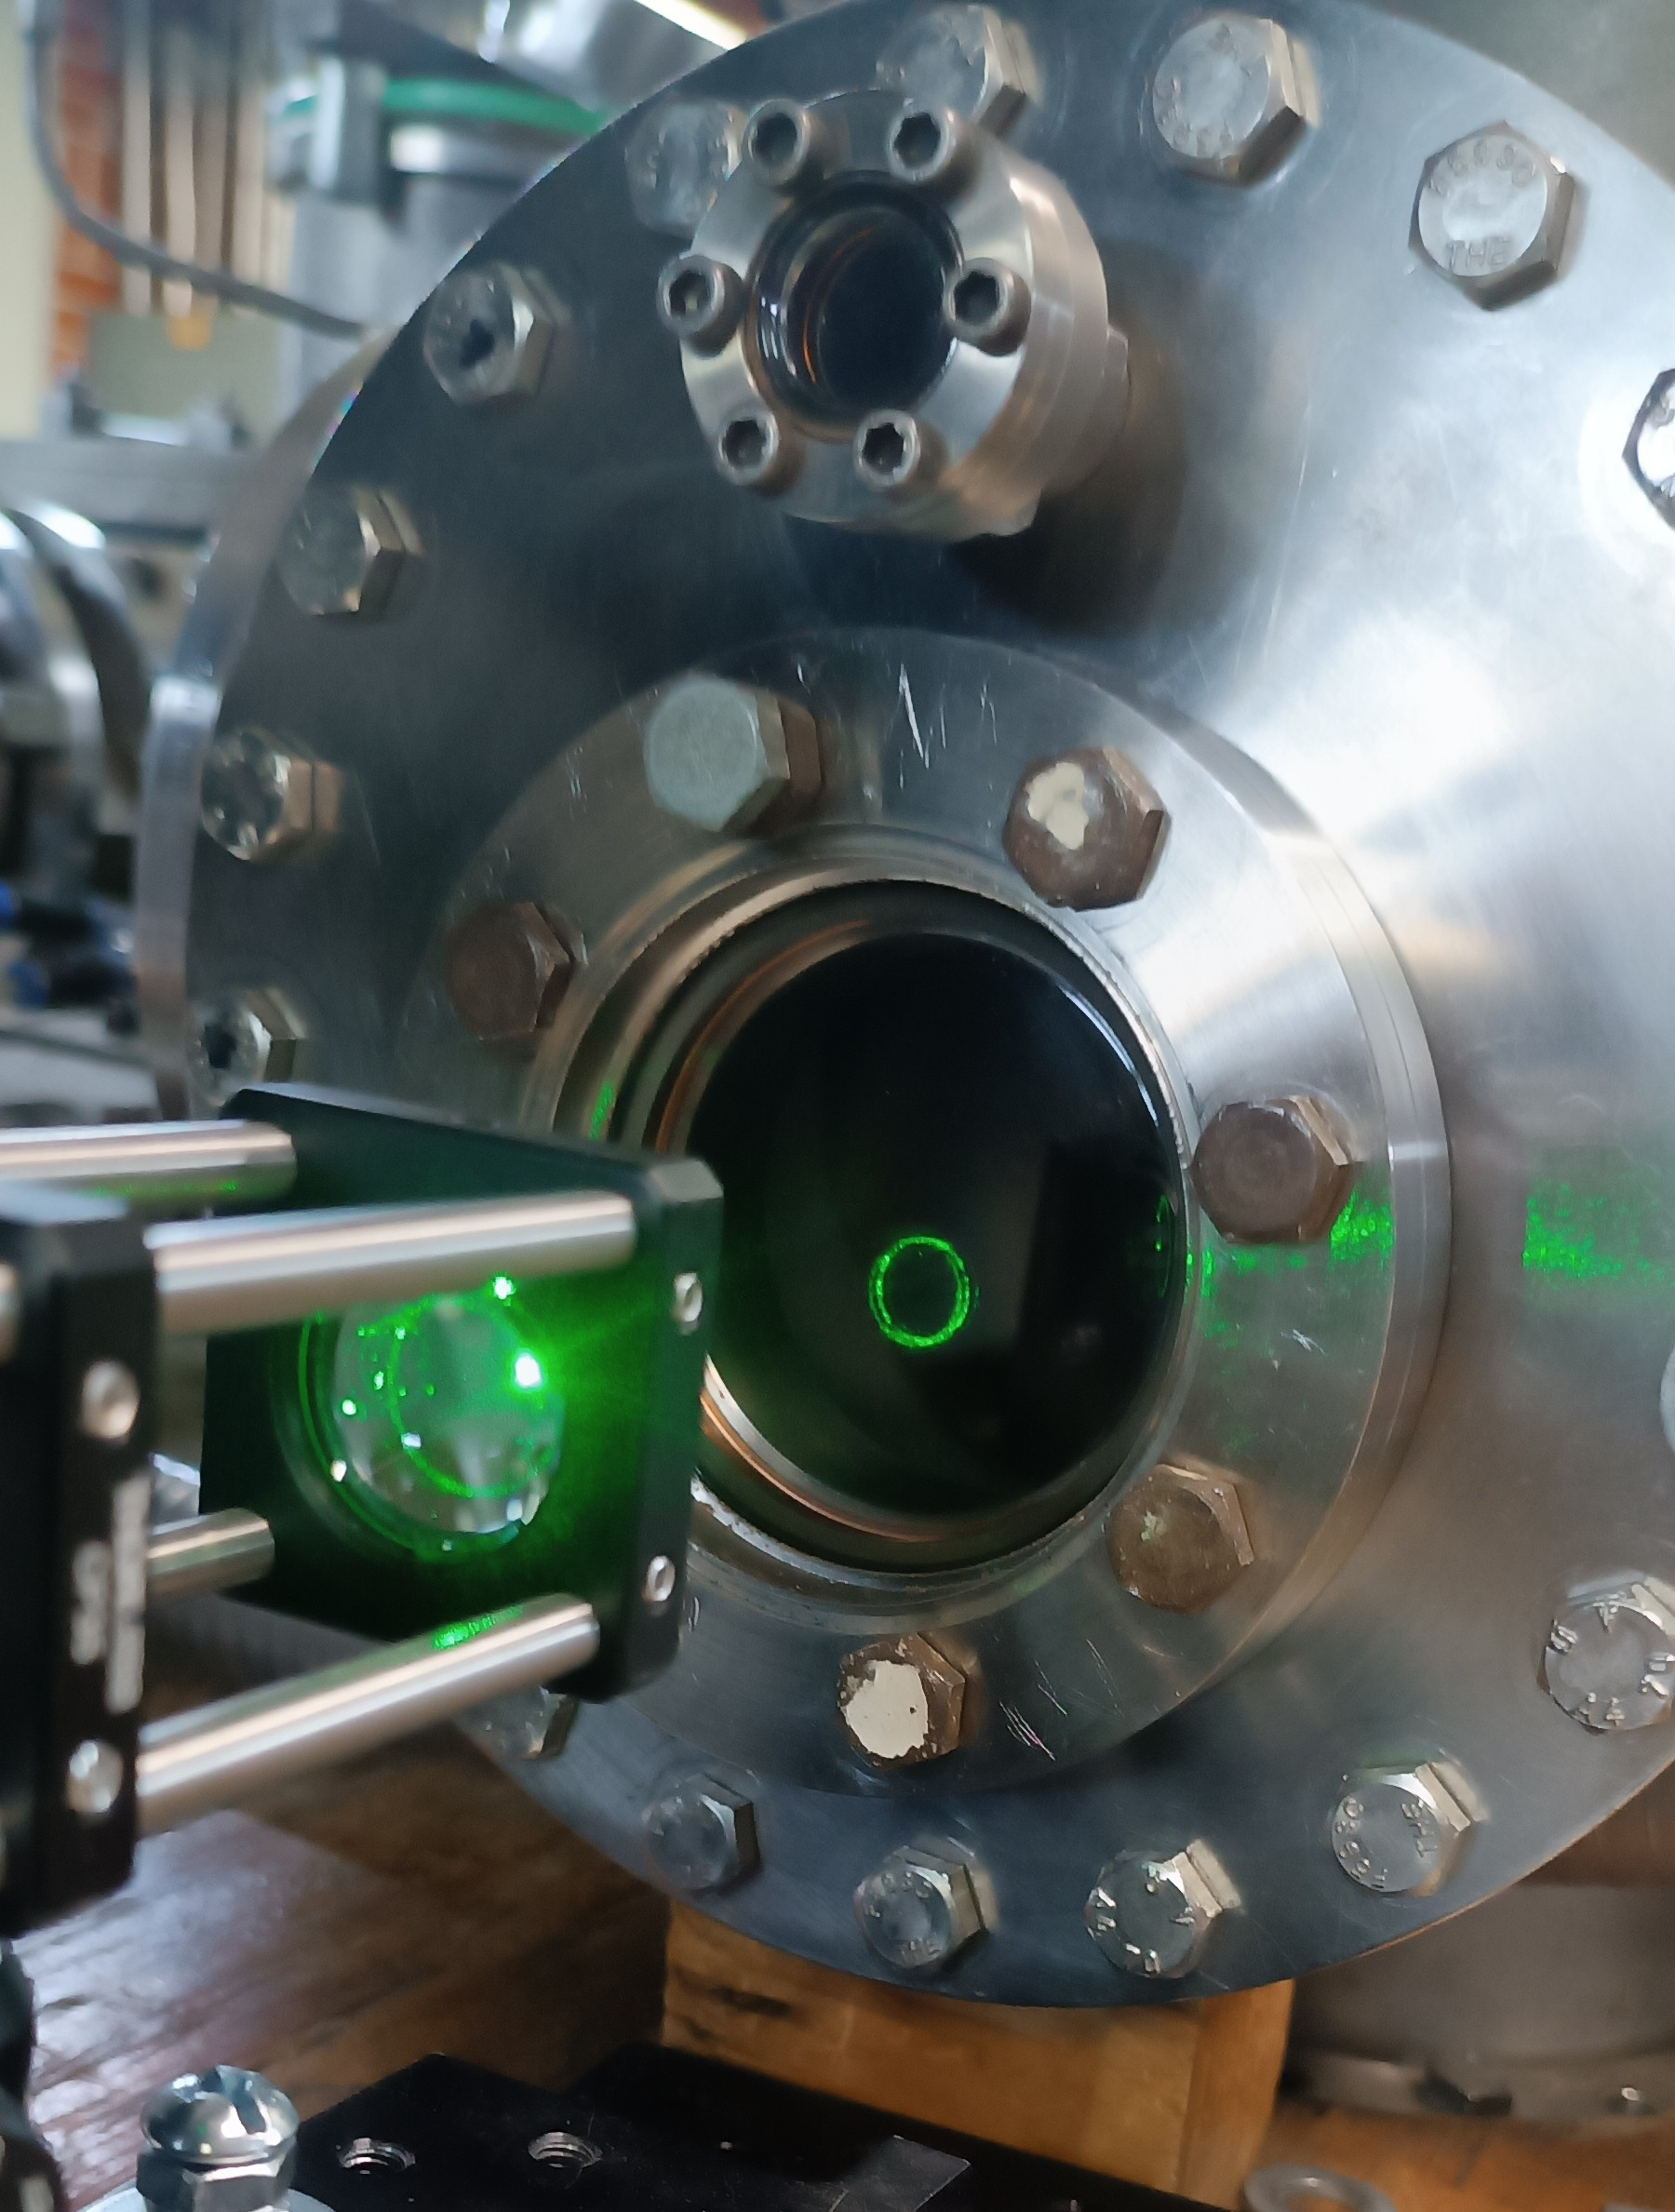
\includegraphics[width=.8\linewidth]{espectrometro-measures.jpg}
	\caption{Espectrómetro óptico colocado en la posición a \qty{6}{\cm} del \emph{racetrack} y \qty{5}{\cm} arriba del blanco \ch{BN}.}
	\label{fig:espectrometro}
\end{figure}

Durante el proceso de deposición, que duró aproximadamente \qty{20}{\min},
se registraron los espectros de emisión en la posición de máxima emisión,
a una altura de \qty{5}{\cm} sobre el blanco de \ch{BN}. En particular,
se realizaron mediciones en distintas etapas del depósito: (a) con el plasma apagado, (b) con e plasma encendido y el \emph{shutter} cerrado, (c) durante el depósito (\emph{shutter} abierto) y (d) al finalizar el depósito.
Las etapas (a) y (c) son de suma importancia, ya que permiten la medición del espectro del fondo, lo cual es esencial para un análisis adecuado de los espectros, ya que el ruido del fondo puede interferir con la identificación de las líneas de emisión de los elementos presentes en el plasma. El plasma que se generó se observa en la \cref{fig:plasma}.

\begin{figure}[htb]
	\centering
	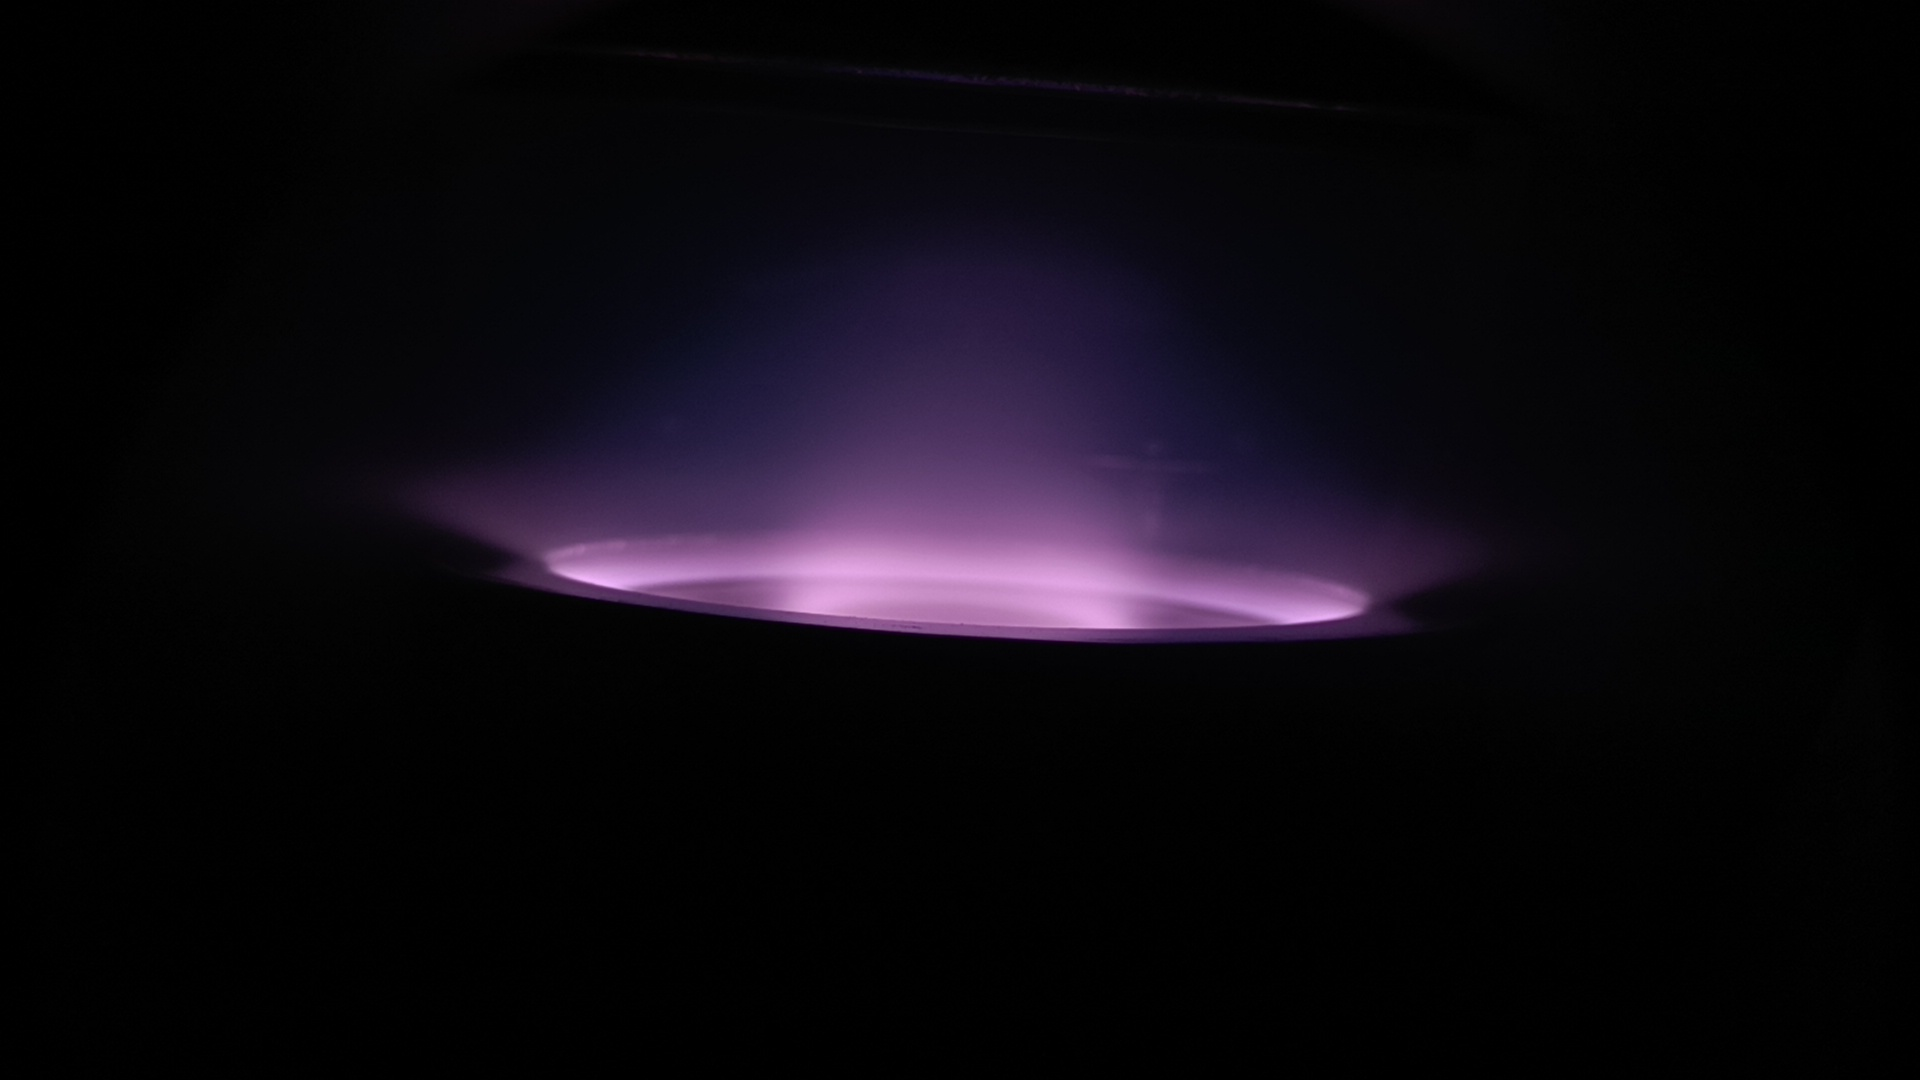
\includegraphics[width=0.9\linewidth]{PLASMA.jpg}
	\caption{Plasma generado durante el depósito de una película delgada de \ch{BN} mediante la técnica rf.}
	\label{fig:plasma}
\end{figure}

\section{Resultados y análisis}

A los espectros obtenidos se les realizó un filtrado con los datos obtenidos
en la etapa (a) para eliminar el ruido de fondo y
así poder identificar las líneas de emisión de los elementos presentes en el plasma.
Para la identificación de las líneas de emisión se usó la base de datos
\emph{NIST Atomic Spectra Database}\cite{nist-asd-lines}, para
extraer los valores correspondientes a los elementos que se esperaban encontrar
en el plasma (\ch{Ar I}, \ch{B I}, \ch{B II} y \ch{N I}) para longitudes de onda entre \qtyrange{200}{900}{\nm}, \cref{fig:emission-lines-complete} Sin embargo, las líneas con intensidades mayores \qty{5000}{a.u.} correspondían únicamente para \ch{B II} y \ch{Ar I}.

\begin{figure}[htp]
	\centering
	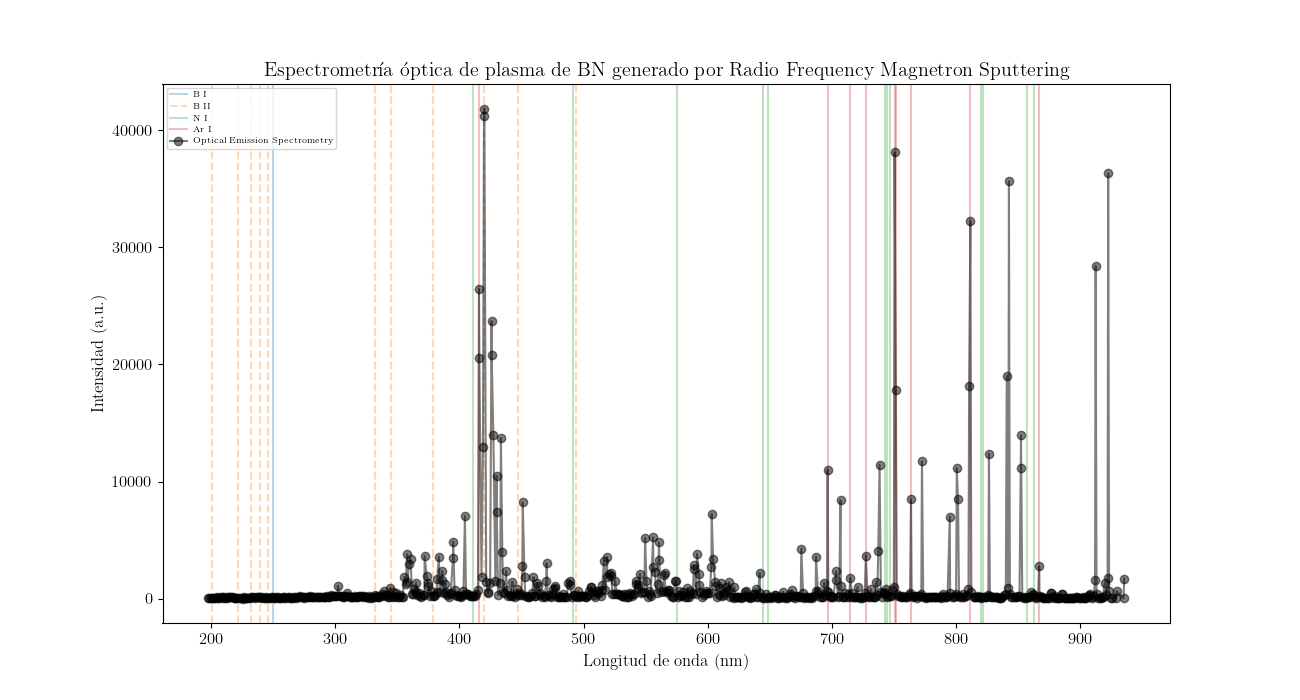
\includegraphics[width=\linewidth]{longitudes_de_onda.png}
	\caption{Espectro del plasma generado durante el depósito con las líneas de emisión para cada uno de los elementos esperados.}
	\label{fig:emission-lines-complete}
\end{figure}

En la \cref{fig:espectro-final} se muestra el espectro después de aplicar el filtrado del fondo, donde se pueden observar las líneas de emisión correspondientes a los elementos con líneas de emisión que superan los \qty{5000}{a.u.} de intensidad.

\begin{figure}[htp]
	\centering
	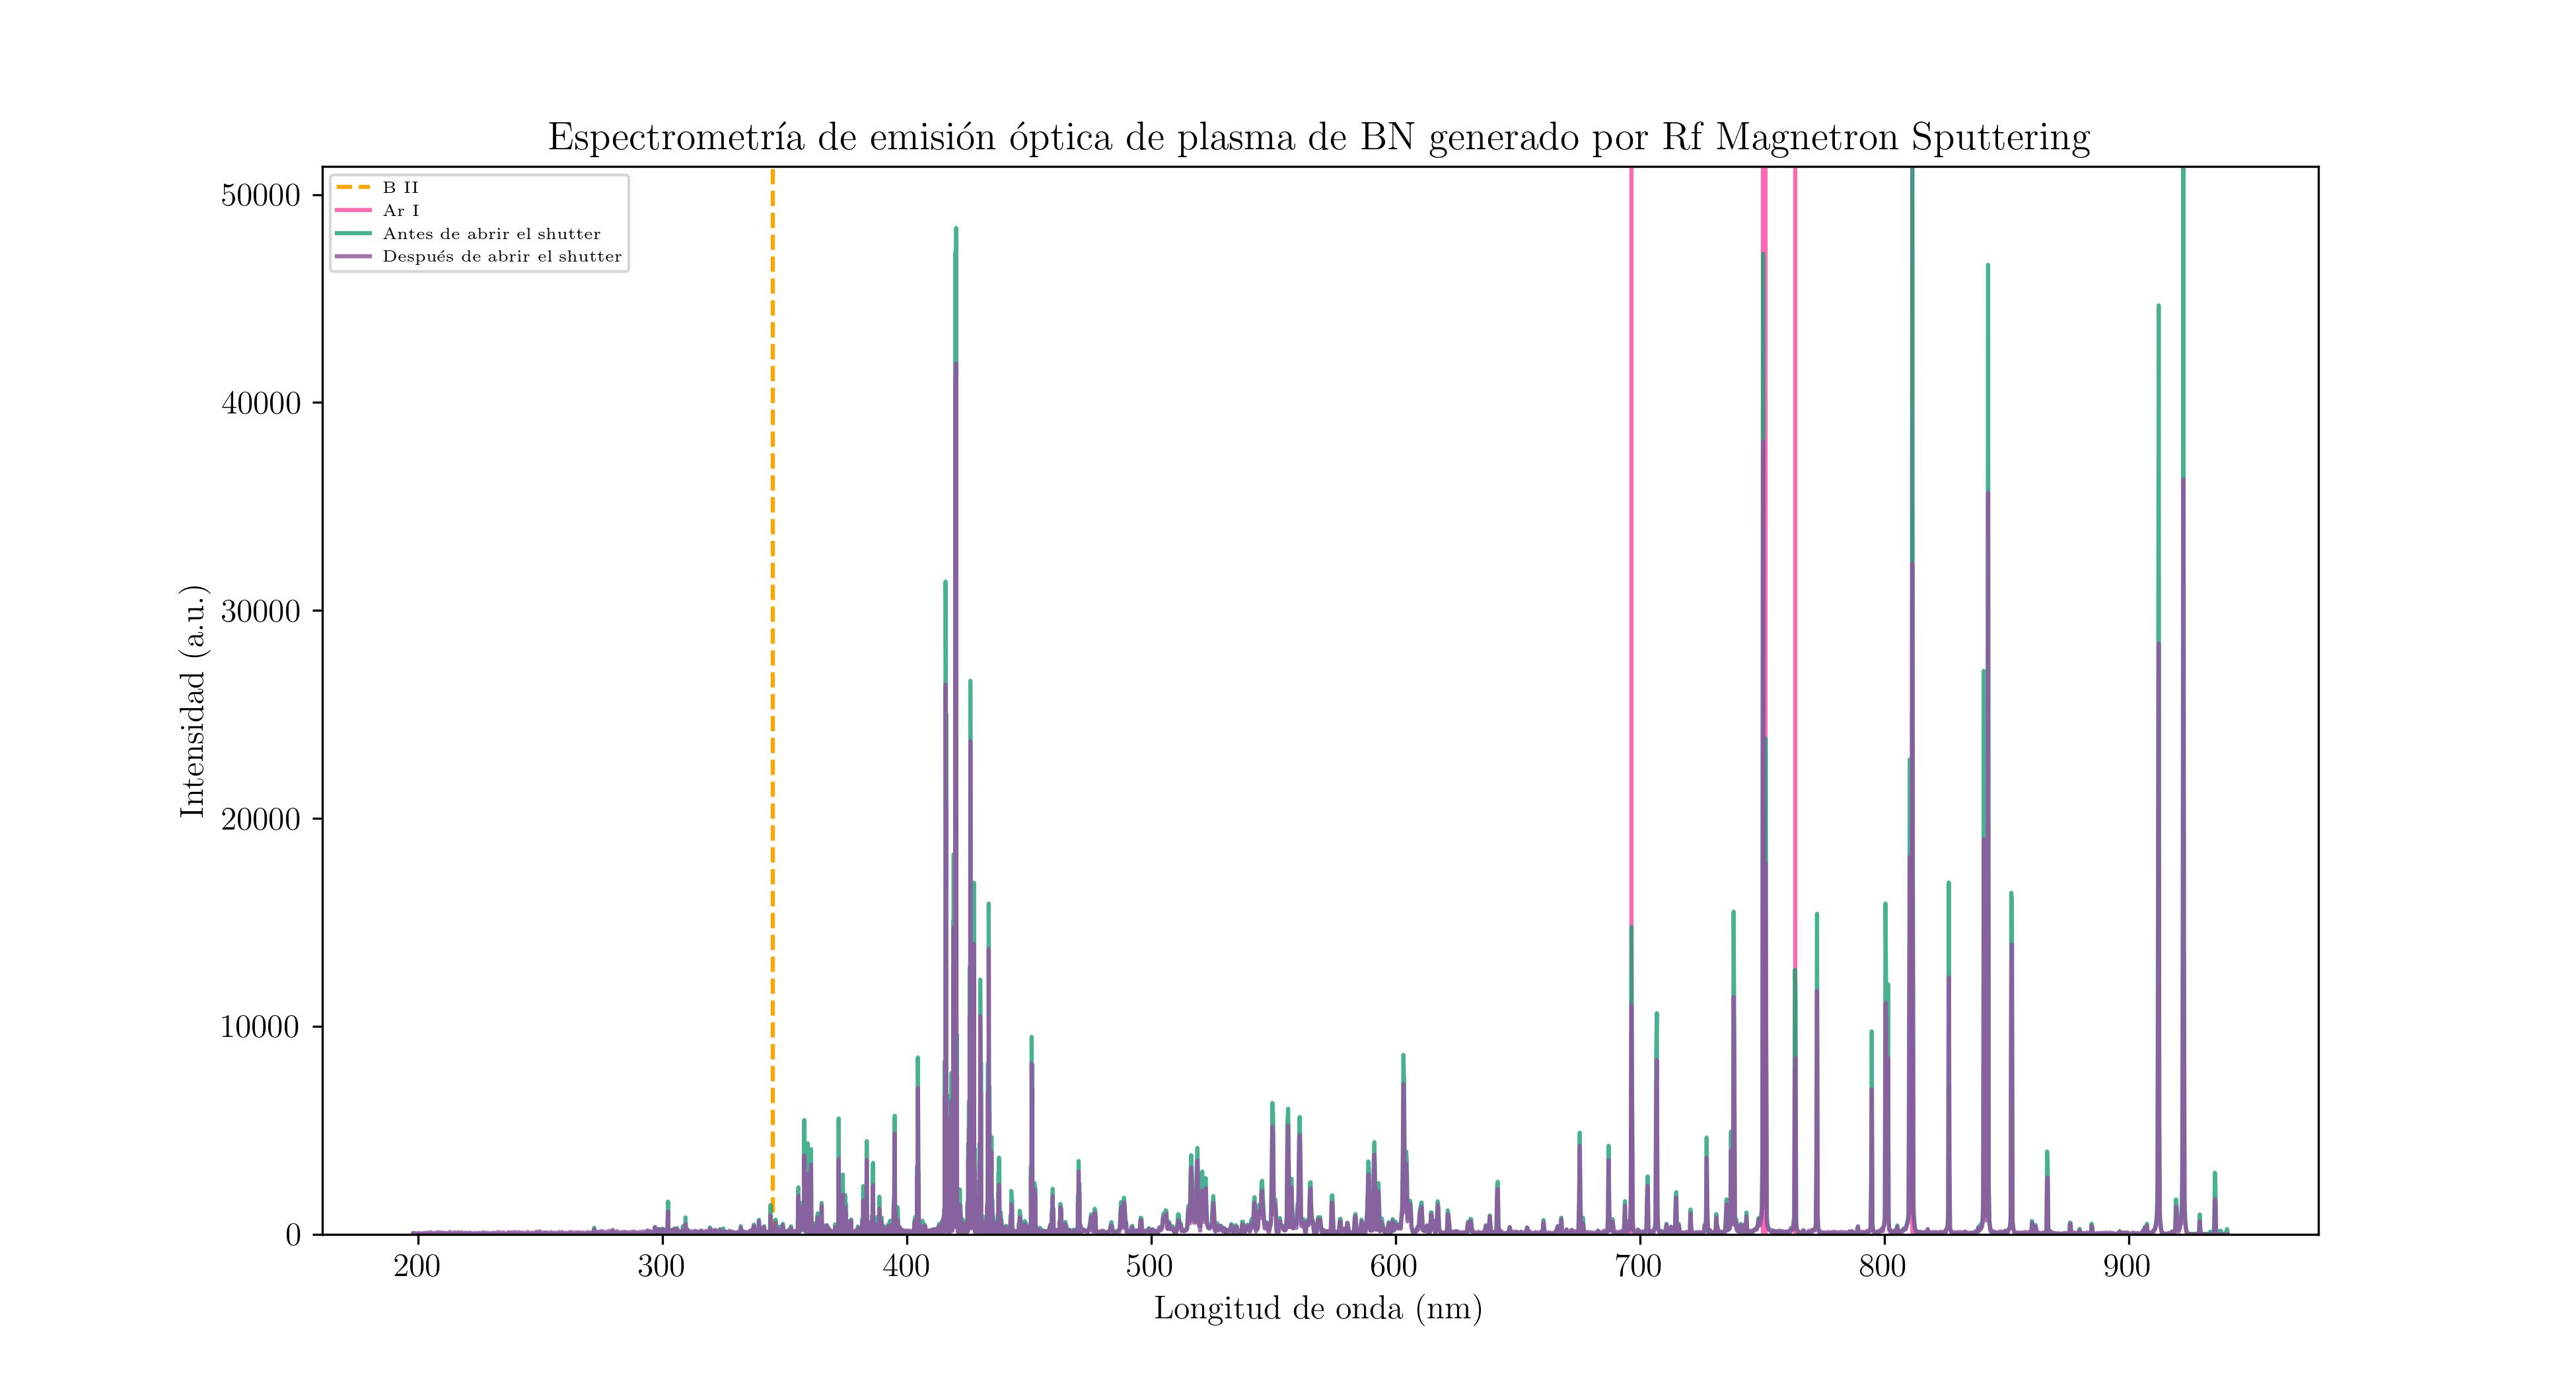
\includegraphics[width=\linewidth]{espectroBN.jpg}
	\caption{Espectro del plasma generado durante el depósito de \ch{BN} con las líneas de emisión filtradas.}
	\label{fig:espectro-final}
\end{figure}



\section{Conclusiones}

El estudio de plasmas generados mediante rf en procesos de deposición de películas delgadas
proporciona información valiosa sobre la dinámica del proceso y la composición elemental
del ambiente de deposición. La técnica de espectroscopía de emisión óptica permitió
identificar las principales líneas de emisión presentes en el plasma generado durante
el depósito de una película delgada de \ch{BN}, destacando las correspondientes a
\ch{Ar I} y \ch{B II}.

Sin embargo, esta técnica trae consigo algunas cuestiones a considerar.
La fibra óptica utilizada requiere de una alineación precisa y un posición fija
durante todo el proceso de adquisición, así como la introducción de ruido de fondo
variable introducido por fuentes externas. Además, el análisis depende del
conocimiento previo sore los elementos esperados, lo que puede limitar la identificación
de otros elementos presentes en el plasma si no se cuenta con esta información.

Si bien se logró un reconocimiento adecuado de las líneas más intensas, la limitación
impuesta a líneas con intensidades mayores a \qty{5000}{a.u.} pudo haber impedido
la identificación de otras líneas relevantes como las de \ch{B I} y \ch{N I}.
Además, es razonable esperar la presencia de líneas de emisión correspondientes a \ch{O I},
debido a la dificultad de eliminarlo completamente en procesos de vacío.

Adicionalmente, sería esperable encontrar trazas de oxígeno (\ch{O}),
ya que es un contaminante común en procesos de deposición en vacío,
incluso después de realizar extracciones de aire.
Su presencia podría confirmarse mediante técnicas complementarias o mediante un umbral
de detección más bajo.

El plasma en sí mismo es un área fascinante de la física con múltiples aplicaciones,
desde la fabricación de dispositivos hasta la astrofísica. Explorar su comportamiento y composición nos permite comprender los procesos de ionización y emisión que lo rigen, abriendo la puerta a mejorar y optimizar diversas tecnologías basadas en plasmas.

En conjunto, este análisis confirma el potencial de la técnica OES para el monitoreo
y caracterización del plasma durante la deposición de películas delgadas,
aunque también señala la importancia de combinarla con otras herramientas
para lograr una caracterización más completa del entorno experimental.
%%%%%%%%%%%%%%%%%%%%%%%%%%%%%%%%
%%%%%%    Bibliografia   %%%%%%%
%%%%%%%%%%%%%%%%%%%%%%%%%%%%%%%%
\nocite{*}
\clearpage
\printbibliography
\end{document}
